%%
%% This is file `sigconf.tex',
%% generated with the docstrip utility.
%%
%% The original source files were:
%%
%% samples.dtx  (with options: `all,proceedings,sigconf')
%% 
%% IMPORTANT NOTICE:
%% 
%% For the copyright see the source file.
%% 
%% Any modified versions of this file must be renamed
%% with new filenames distinct from sigconf.tex.
%% 
%% For distribution of the original source see the terms
%% for copying and modification in the file samples.dtx.
%% 
%% This generated file may be distributed as long as the
%% original source files, as listed above, are part of the
%% same distribution. (The sources need not necessarily be
%% in the same archive or directory.)
%%
%%
%% Commands for TeXCount
%TC:macro \cite [option:text,text]
%TC:macro \citep [option:text,text]
%TC:macro \citet [option:text,text]
%TC:envir table 0 1
%TC:envir table* 0 1
%TC:envir tabular [ignore] word
%TC:envir displaymath 0 word
%TC:envir math 0 word
%TC:envir comment 0 0
%%
%% The first command in your LaTeX source must be the \documentclass
%% command.
%%
%% For submission and review of your manuscript please change the
%% command to \documentclass[manuscript, screen, review]{acmart}.
%%
%% When submitting camera ready or to TAPS, please change the command
%% to \documentclass[sigconf]{acmart} or whichever template is required
%% for your publication.
%%
%%
\documentclass[sigconf]{acmart}
%%
%% \BibTeX command to typeset BibTeX logo in the docs
\AtBeginDocument{%
  \providecommand\BibTeX{{%
    Bib\TeX}}}

%% Rights management information.  This information is sent to you
%% when you complete the rights form.  These commands have SAMPLE
%% values in them; it is your responsibility as an author to replace
%% the commands and values with those provided to you when you
%% complete the rights form.
%\setcopyright{acmlicensed}
%\copyrightyear{2026}
%\acmYear{2026}
%\acmDOI{XXXXXXX.XXXXXXX}
%% These commands are for a PROCEEDINGS abstract or paper.
%\acmConference[MODELS 2026]{ACM/IEEE 29th International Conference on Model Driven Engineering Languages and Systems (MODELS)}{4-9 October 2026}{ Málaga, Spain}
%%
%%  Uncomment \acmBooktitle if the title of the proceedings is different
%%  from ``Proceedings of ...''!
%%
%%\acmBooktitle{Woodstock '18: ACM Symposium on Neural Gaze Detection,
%%  June 03--05, 2018, Woodstock, NY}
%\acmISBN{978-1-4503-XXXX-X/2018/06}

\copyrightyear{2026}
\acmYear{2026}
\setcopyright{cc}
\setcctype{by}
\acmConference[MODELS 2026]{ACM/IEEE 29th International Conference on Model Driven Engineering Languages and Systems}{October 04--09, 2026}{Málaga, Spain}
\acmBooktitle{ACM/IEEE 29th International Conference on Model Driven Engineering Languages and Systems (MODELS 2026), October 04--09, 2026, Málaga, Spain}
\acmDOI{10.1145/3822455.3838774}
\acmISBN{979-8-4007-2809-9/2026/10}




%%
%% Submission ID.
%% Use this when submitting an article to a sponsored event. You'll
%% receive a unique submission ID from the organizers
%% of the event, and this ID should be used as the parameter to this command.
%%\acmSubmissionID{123-A56-BU3}

%%
%% For managing citations, it is recommended to use bibliography
%% files in BibTeX format.
%%
%% You can then either use BibTeX with the ACM-Reference-Format style,
%% or BibLaTeX with the acmnumeric or acmauthoryear sytles, that include
%% support for advanced citation of software artefact from the
%% biblatex-software package, also separately available on CTAN.
%%
%% Look at the sample-*-biblatex.tex files for templates showcasing
%% the biblatex styles.
%%
%%
%% The majority of ACM publications use numbered citations and
%% references.  The command \citestyle{authoryear} switches to the
%% "author year" style.
%%
%% If you are preparing content for an event
%% sponsored by ACM SIGGRAPH, you must use the "author year" style of
%% citations and references.
%% Uncommenting
%% the next command will enable that style.
%%\citestyle{acmauthoryear}


\usepackage{xcolor}
\usepackage{xspace}
\usepackage{multirow} % in preamble
\usepackage{booktabs} % in preamble
\usepackage{array} % in preamble



\long\def\red#1{{\color{red}#1}}
\newcommand{\cc}[1]{{\small{\tt #1}}}
\newcommand{\rf}{\textcolor{red}{[C]}\xspace}
\newcommand{\rc}[1]{\textcolor{red}{[#1]}\xspace}
\newcommand{\R}{{\mathbb R}} 
\newcommand{\ff}{\hspace{-0.1em}f}

\newcommand{\repo}{repo-name}


%%
%% end of the preamble, start of the body of the document source.
\begin{document}

%%
%% The "title" command has an optional parameter,
%% allowing the author to define a "short title" to be used in page headers.
\title{Can LLMs Substitute for Humans in Evaluating Conceptual Modeling Language Vocabularies? An Experimental Study}

%%
%% The "author" command and its associated commands are used to define
%% the authors and their affiliations.
%% Of note is the shared affiliation of the first two authors, and the
%% "authornote" and "authornotemark" commands
%% used to denote shared contribution to the research.
\author{Ghazal Rafati}
\email{ghazalrs@my.yorku.ca}
\orcid{0009-0006-7726-1032}
\affiliation{%
  \institution{
  Department of Electrical Engineering and Computer Science \\ 
  York University}
  \city{Toronto}
  \state{ON}
  \country{Canada}
}


\author{Anthony Romaniello}
\email{anthromaniello@gmail.com}
\orcid{0009-0007-2751-8247}
\affiliation{%
  \institution{
  School of Information Technology \\ 
  York University}
  \city{Toronto}
  \state{ON}
  \country{Canada}
}


\author{Sotirios Liaskos}
\correspondingauthor
\email{liaskos@yorku.ca}
\orcid{0000-0001-5625-5297}
\affiliation{%
  \institution{
  School of Information Technology \\ 
  York University}
  \city{Toronto}
  \state{ON}
  \country{Canada}
}



%%
%% By default, the full list of authors will be used in the page
%% headers. Often, this list is too long, and will overlap
%% other information printed in the page headers. This command allows
%% the author to define a more concise list
%% of authors' names for this purpose.
\renewcommand{\shortauthors}{Rafati, Romaniello, and Liaskos}

%%
%% The abstract is a short summary of the work to be presented in the
%% article.
\begin{abstract}
Effective model-driven engineering of software-intensive systems relies on appropriately designed conceptual modeling languages. A well-designed modeling language includes a set of concepts that users of the language find to be relevant for describing phenomena of interest in a domain, as well as a vocabulary of lexical, symbolic, or visual signifiers for representing these concepts. 
Being the product of a human design process, however, a modeling language may or may not feature the optimal choice of concepts and signifiers. 
One of the ways that have been proposed to assess the quality of those choices is based on requesting potential users of the language to use it for classifying a sample of chunks of information from an example domain under one or more of the proposed concepts of the language. Characteristics of the classification results, such as agreement among users and between users and authoritative classifications, are revealing of the quality of the chosen set of concepts and their signifiers. In this paper, we report on an experimental investigation in using Large Language Models (LLMs) as substitutes for human input in such classifications to allow rapid, cost-effective acquisition of quality data. Specifically, using an example subject language, we compare the accuracy of human versus LLM classifications with respect to authoritative standards. We find that LLM performance in the specific tasks is substantially higher than human performance, challenging the idea that LLMs can be readily used to simulate human performance for such tasks. We discuss the implications of this early finding for future research.
\end{abstract}

%%
%% The code below is generated by the tool at http://dl.acm.org/ccs.cfm.
%% Please copy and paste the code instead of the example below.
%%
\begin{CCSXML}
<ccs2012>
   <concept>
       <concept_id>10011007.10011006.10011050.10011017</concept_id>
       <concept_desc>Software and its engineering~Domain specific languages</concept_desc>
       <concept_significance>500</concept_significance>
       </concept>
   <concept>
       <concept_id>10011007.10011006.10011050.10011023</concept_id>
       <concept_desc>Software and its engineering~Specialized application languages</concept_desc>
       <concept_significance>500</concept_significance>
       </concept>
   <concept>
       <concept_id>10002944.10011123.10010912</concept_id>
       <concept_desc>General and reference~Empirical studies</concept_desc>
       <concept_significance>500</concept_significance>
       </concept>
   <concept>
       <concept_id>10002944.10011123.10010916</concept_id>
       <concept_desc>General and reference~Measurement</concept_desc>
       <concept_significance>500</concept_significance>
       </concept>
 </ccs2012>
\end{CCSXML}

\ccsdesc[500]{Software and its engineering~Domain specific languages}
\ccsdesc[500]{Software and its engineering~Specialized application languages}
\ccsdesc[500]{General and reference~Empirical studies}
\ccsdesc[500]{General and reference~Measurement}


%% A "teaser" image appears between the author and affiliation
%% information and the body of the document, and typically spans the
%% page.
\begin{comment}
\begin{teaserfigure}
 \includegraphics[width=\textwidth]{sampleteaser}
  \caption{Seattle Mariners at Spring Training, 2010.}
  \Description{Enjoying the baseball game from the third-base
  seats. Ichiro Suzuki preparing to bat.}
  \label{fig:teaser}
\end{teaserfigure}
\end{comment}

%\received{1 July 2026}
%\received[revised]{12 March 2009}
%\received[accepted]{5 June 2009}

%%
%% This command processes the author and affiliation and title
%% information and builds the first part of the formatted document.
\maketitle


\section{Introduction}

% The imprtance of language and what they do.

Model-driven engineering of software-intensive systems is heavily based on the definition and use of \textit{conceptual modeling languages}. Such languages prescribe how modelers are supposed to build models and how readers are meant to understand those models. A well-designed conceptual modeling language supports the efficient development of comprehensible conceptual models that are usable in different activities of the engineering lifecycle, including stakeholder communication, decision making, validation and verification, and code generation.

% Constitutents of Languages
The heart of a modeling language is an \textit{ontology} that captures a shared \textit{conceptualization} of a domain among language users \cite{Guiz.07}. The constituents of the ontology are \textit{concepts} which are used to organize the apprehension and communication of pertinent phenomena in the domain. In the language, concepts are represented through \textit{terms}, i.e., lexical, symbolic, and/or visual elements that represent concepts. UML state diagrams \cite{UML.17}, for example, are models that are based on a language containing such concepts as \textit{state}, \textit{transition}, and \textit{guard condition}, represented lexically in English through a \textit{vocabulary} of terms, such as ``state'', ``transition'', ``guard condition'', as well as designated visual elements, such as rounded rectangles, arrows, and bracketed annotations on arrows. For simplicity we will, henceforth, refer to any kind of signification of concepts (lexical, visual, or other) as \textit{terms}. 

% The design problem
%Conceptual modeling languages are artifacts, embodying a series of design decisions made by the language designers. These decisions involve, among other things, 

The selection of concepts that should be included in the language and the terms for representing those concepts, are the result of a design effort. As in any design effort, the outcome can enjoy different degrees of success as reflected by the \textit{quality} of the resulting modeling language. In recognition of this, several efforts to conceptualize language quality can be found in the literature \cite{Krog.12,NePG.12,WeWa.93}. Key focus has been the \textit{appropriateness} of a chosen vocabulary vis-a-vis the concepts of the underlying ontology it is intended to represent -- often referred to as \textit{semantic transparency} \cite{Mood.10} seen as part of the language's general \textit{comprehensibility appropriateness} \cite{Krog.12}. Wand and Weber, specifically, introduce a framework for characterizing pathologies of language designs based on how exactly the vocabulary-ontology mapping is missaligned \cite{WeWa.93}. For example, a language suffers from \textit{construct deficit} when there are concepts in the language that are not represented by corresponding terms in the vocabulary, and, reversely, \textit{construct excess}, when there are terms not obviously mapping to a concept of interest.

% The peira approach
With the dimensions of vocabulary quality theoretically defined in such a way, the natural question is how one can measure a given language design with respect to each of those dimensions. An empirical approach for doing so has been proposed by Liaskos et al. \cite{LZMK.24}. According to their framework, called \textit{Peira}, such assessments are possible via exposing experimental participants to chunks of ``raw'' unstructured domain information and asking them to classify such chunks to terms of the language vocabulary under investigation, after first exposing them to the language through a training process of specified length, depth, and intensity. The outcomes of the classification are then used to calculate a variety of metrics either based on comparison to authoritative classifications, i.e., classifications claimed to be correct by the vocabulary designers themselves, or, ignoring authoritative input, based on measures of agreement among the participants. The authors go on to propose specific formulae by which the resulting classification datasets can be used to detect the presence of language issues such as the ones discussed above -- construct deficit, construct excess, etc. 
%\red{According to the authors, the process is meant to streamline language design evaluation allowing evaluators to utilize a common set of metrics, enable comparisons between designs under certain assumptions, and avoid the subjectivity and biases lurking in alternative procedures, such as expert evaluation of complete models.}

The process is, however, not without cost given that a number of human participants need to be recruited, trained to the language, and engage in classification tasks. With the advent of Large Language Models (LLMs) \cite{LLM.survey} it is, hence, pertinent to ask whether LLMs can be used as a substitute for human participants. Specifically, instead of training humans and asking them to perform classification tasks, present the training material to an LLM and subsequently ask the LLM to perform the classification tasks instead -- all within one or a sequence of prompts. For such a strategy to be applicable at least two issues need to be clarified: (a) whether LLM performance is comparable with human performance to allow for such substitution and (b) whether the choice of LLM affects such performance and substitutability. 

In this paper, we report on a preliminary empirical study in which the Peira framework is applied with both humans and LLMs, as a first attempt to address the above questions
% via a direct comparison between the two kinds of participants. 
An example requirements modeling language that was recently introduced in the literature is adopted as the object of investigation. The Peira method is applied using on-line participants who complete a sequence of tasks in a survey-style on-line instrument, as prescribed by the method. 
%The latter consists of video presentations of the language in question as well as other instructions followed by classification tasks based on two distinct cases. 
The instrument is then converted to an LLM prompt that conveys, to the extend feasible,
% via verbatim transcription of the training video and adaptation of question and response inventory format to prompt design conventions, 
the exact same information as the on-line instrument. The LLM prompt is offered to a set of LLMs with different sizes. The resulting data sets are compared with respect to classification performance, i.e., the levels of precision and recall attained by human vs. LLM ratings when compared to authoritative ratings. We find that LLMs substantially outperform humans, preventing them to be trivially used as substitutes of the latter, and, that, moreover, the more the parameters of the LLM the better its performance.

The rest of the paper is organized as follows. In Section \ref{sec:background}, we review the Peira framework. In Section \ref{sec:study}, we describe the experimental study. In Section \ref{sec:related} we offer a brief survey of related work and conclude in Section \ref{sec:conclusions} with future directions.




\section{The Peira framework}\label{sec:background}

Peira is a framework for systematic conduct of experimental studies for the purpose of evaluating the appropriateness of conceptual modeling language vocabularies \cite{LZMK.24}. An instance of a Peira experiment is meant to evaluate a set $V$ of \textit{signifiers} representing the vocabulary of the language to be evaluated. To do so, a sample of descriptions $E$ is taken from one or more application domains where the language is meant to be used. Further, a set of $\mathbf{D} = D \cup R$ of distinguished elements $D$ from each domain, combined with a set of $R$ n-tuples thereof, are defined as a sample of the Universe of Discourse (UoD) relating to the domain and deemed as worthy of being modeled using the vocabulary. Domain elements from $\mathbf{D}$ under specific descriptions are referred to as \textit{subjects} from a set $S = \mathbf{D} \times E$. A set $P$ of \textit{raters} are also identified as a sample (or a proxy thereof) from a population of potential users of the language whose vocabulary is in question. The role of the raters is to study each description  $e\in E$ and classify each subject $s\in S$ associated with $e$ to none, one, or more of the terms in vocabulary $V$.

As an example, consider a simple domain-specific language for describing enrollment and attendance of students to courses and lectures, using concepts \textit{course}, \textit{student}, \textit{lecture}, (entities / unary concepts) \textit{enrolls}, \textit{includes lecture}, and \textit{attends lecture} (relationships / binary concepts). Our evaluation question is if the vocabulary $V = $ \{``course'', ``student'', ... \} --- the English words representing the above concepts --- is appropriate for describing situations involving students enrolling courses, attending lectures, etc. A set of descriptions $E$ is prepared of real or contrived cases of students taking courses, attending lectures etc. Consider that in one of them $e\in E$, Alice decided to take Statistics only to find that it is hard to follow and that she fell asleep during the lecture on the Central Limit Theorem (CLT). Within the context of the case, elements of  $D$ include ``Alice'', ``Statistics'', ``Lecture on CLT'' and elements of $R$ include tuples such as ``(Alice, Statistics)'', ``(Alice, Lecture on CTL)'', and ``(Statistics, Lecture on CTL)''. These elements combined constitute subjects $s\in S$ under the description of Alice's case $e$. These subjects are to be classified under none, one, or more of the elements in $V$ by a sample of participants who are likely to use the vocabulary, such as the maintainers and analysts/instantiators of a software product line for course enrollment and attendance tracking.

The result of the classification exercises is a dataset of triples $(p,s,v)$ --- rater $p$ classified subject $s$ under term $v$ --- which Peira proposes can be the basis for several metrics of assessing different qualities of the vocabulary, assuming representativeness of descriptions, subjects, and raters. For example, when a term $v$ is rarely or never featured in any triple, this can be construed as evidence of construct excess: $v$ could be dropped from the language. Reversely, subjects $s\in S$ not appearing in any triples could be evidence of construct deficit: while the experimenters thought that $s$ is worthy of being modeled, hence included in $S$, the participants could not classify it under any of the available terms. The authors offer concrete formulae for quantitatively expressing those issues \cite{LZMK.24}. 

For simplicity, we will, here, focus on Peira metrics that compare participant responses with the authoritative classifications, i.e., the complete set of $(p_a,s,v)$ triples that the language designers believe are valid classifications. Following \cite{LZMK.24} let function $n: P\times S \times V \mapsto \{0,1\}$, be $n(p,s,v) = 1$ if participant $p$ has offered classification $(p,s,v)$, and $n(p,s,v) = 0$ otherwise. Let now $p_a$ be a participant from $P$ that holds the authoritative response. Define the following for $p\neq p_a$:
\[ 
\mathit{acc}(p,s,v)= \left\{
\begin{array}{ll}
	\mathbf{1}, \:\mathrm{if}\,n(p_a,s,v) = 1\,\mathrm{and}\,n(p,s,v) = 1\\
	\textbf{0}, \:\mathrm{otherwise} \\
\end{array} 
\right. 
\]
\[
\mathit{def}(p,s,v)= \left\{
\begin{array}{ll}
	\mathbf{1}, \:\mathrm{if}\,n(p_a,s,v) = 1\,\mathrm{and}\,n(p,s,v) = 0\\
	\textbf{0}, \:\mathrm{otherwise} \\
\end{array} 
\right. 
\]
\[
\mathit{exc}(p,s,v)= \left\{
\begin{array}{ll}
	\mathbf{1}, \:\mathrm{if}\,n(p_a,s,v) = 0\,\mathrm{and}\,n(p,s,v) = 1\\
	\textbf{0}, \:\mathrm{otherwise} \\
\end{array} 
\right. 
\]

We further use $\mathit{acc}(\cdot,\cdot,v)$, $\mathit{def}(\cdot,\cdot,v)$, and 
$\mathit{exc}(\cdot,\cdot,v)$ to represent the marginal totals for each term over all subjects and all participants, e.g., $\mathit{acc}(\cdot,\cdot,v) = \sum_{p\in {P \setminus {p_a}}}\sum_{s\in S} \mathit{acc(p,s,v)}$. According to Peira, the quantities offer raw measures of the {\em accuracy}, {\em scope deficiency} and {\em scope excess} of a given term. Specifically, for a specific term $v$, $\mathit{acc}(\cdot,\cdot,v)$ represents the number of ratings in which participants and designers are in agreement with respect to term $v$, $\mathit{def}(\cdot,\cdot,v)$ the number of authoritative ratings that were not picked by participants (``false negatives''), and $\mathit{exc}(\cdot,\cdot,v)$ the participant ratings that are in excess of the authoritative ones (``false positives''). It follows that, in the more familiar terms of precision and recall:

\noindent $\mathrm{prec}^{pc}_V(v) = acc(\cdot,\cdot,v)/(acc(\cdot,\cdot,v)+exc(\cdot,\cdot,v))$

\noindent $\mathrm{rec}^{pc}_V(v) = acc(\cdot,\cdot,v)/(acc(\cdot,\cdot,v)+def(\cdot,\cdot,v))$

Seeing participants as classifiers of labeled data (the authoritative classifications), the above describe the \textit{precision-per-concept} and \textit{recall-per-concept} of the corresponding classification exercise. Concepts for which these metrics are comparatively low are subjects for investigation by designers.

Likewise, $\mathit{acc}(p,\cdot,\cdot)$, $\mathit{def}(p,\cdot,\cdot)$, and $\mathit{exc}(p,\cdot,\cdot)$ offer corresponding measures characterizing the input of a specific participant compared to the authoritative. These ratings measure the degree to which the participant is in general agreement with the designers vis-a-vis the vocabulary, and characterize the performance of that participant. In terms of precision and recall again:

\noindent $\mathrm{prec}^{pp}_V(p) = acc(p,\cdot,\cdot)/(acc(p,\cdot,\cdot)+exc(p,\cdot,\cdot))$

\noindent $\mathrm{rec}^{pp}_V(p) = acc(p,\cdot,\cdot)/(acc(p,\cdot,\cdot)+def(p,\cdot,\cdot))$

These metrics are called \textit{precision-per-participant} and \textit{recall-per-participant} and are used in Peira to also evaluate the language in a way that is amenable to statistical inferences. Below we will use these metrics to compare participant performance.

While Peira is agnostic to how experimenters acquire ratings in practice, in their experiments, the authors have utilized questionnaire-style instruments in which participants, after being shown training videos, are presented a case, followed by a presentation of subjects below each of which a multi-choice inventory of vocabulary terms (plus the ``None'' option) are offered for participants to classify the subject under one or more terms \cite{LZMK.24}. In the experimental study we followed the same rating acquisition style, as we describe below.

\section[Experimental Study]{Experimental Study\protect\footnote{Reproducibility package: https://github.com/anonymous-author-1000/auto-peira/}}\label{sec:study}

\subsection{Motivation and Goals}

The Peira process is based on recruiting, training, and having experimental participants perform rating tasks. This entails cost and effort for those involved. With the advent of Large Language Models (LLMs) \cite{LLM.survey} the question of whether such models can act as more accessible and cost-effective proxies for human input becomes relevant. At the same time, as increased LLM size is known to improve capability but also increase computational cost and environmental impact, it is also useful to know how small an LLM can be and still play the role of a faithful substitute for human participants. The experimental study we report below addresses these research goals. The specific research questions (RQs) are:

\textbf{RQ1.} Can LLMs be used as substitutes for human raters in Peira?

\textbf{RQ2.} Does model size affect the performance of LLMs in executing Peira's rating tasks?

To answer these questions, we apply Peira on a chosen modeling language in two ways: (a) with human participants performing the ratings, as proposed by the method, and (b) with LLMs performing the ratings instead. To assess whether LLMs perform at human level so as to justify their use as substitutes for human raters (RQ1), we measure and compare the rating performance, in terms of precision and recall with respect to the authoritative ratings, of LLMs vs. humans. For LLMs to be considered an appropriate substitute for humans for the task, we require that their performance falls within a confidence interval of average human performance; otherwise, if LLMs perform significantly better or worse than humans, they cannot be considered faithful proxies of human judgment for this task. Furthermore, the LLMs are sampled to be of different sizes with respect to their number of parameters in order to allow size to be investigated as a predictor of performance in the classification tasks (RQ2).

\subsection{Study Design}

\subsubsection{Language}

For our study we choose a language recently introduced in the literature for modeling reinforcement learning domains \cite{LKMG.24}. The language, called iStar-DT, is an extension of iStar 2.0 \cite{DaFH.16}, a language for intentional modeling of socio-technical systems. The original iStar 2.0 includes entities (unary concepts) such as \textit{actors}, which are participants in the socio-technical system in question, \textit{goals} adopted and pursued by said actors, \textit{tasks}, which describe specific actions performed by actors to pursue their goals, and \textit{qualities}, which describe attributes that actors want to be satisfied while attaining goals. Relationships include \textit{AND-} and \textit{OR-decompositions} of goals into subgoals and tasks, and  \textit{contribution links} that show how satisfaction of goals, tasks, or qualities affect satisfaction of other qualities. 

The iStar-DT extension adds concepts for modeling the state of the environment in which actors pursue their goals as well as to express temporal constraints in task execution and goal satisfaction. Thus, \textit{affects} relationships connect tasks with \textit{effect} elements showing how tasks affect the state of the environment, and \textit{precedes} relationships express that performance of a task requires prior performance or satisfaction of another task or goal.  The extension also introduces \textit{pre-effect} and \textit{pre-quality} elements to represent the state of effects and qualities at a specified previous time. A visual notation is also proposed to diagrammatically signify these concepts.

The details of iStar-DT are beyond the scope of this presentation; readers can refer to the publication introducing it \cite{LKMG.24}. Interestingly, the authors' most recent publication \cite{LDKM+26} features updates and simplifications to the iStar-DT ontology. In this study, we adopt their original proposal \cite{LKMG.24}, without harming our research strategy. Overall, the vocabulary $V$ under investigation includes 18 elements, 9 of which are entities (unary concepts, e.g. ``goal'', ``task'', etc.) and the remaining 9 are relationships (binary concepts, e.g., ``affects'', ``positively contributes to'', etc.). 

\subsubsection{Instrument and Tasks for Human Participants}

With the language under investigation selected, we next develop the rating acquisition instrument, according to the Peira specifications. The instrument is administered online and consists of a sequence of screens in which participants perform various tasks as follows. A video welcoming participants and outlining the engagement is first presented, followed by a 15 minute video presentation of iStar-DT. This, in turn, is followed by a screen with video comprehension exercises, to be used for filtering inattentive participants. Next, participants are given a list of selected pairs of iStar-DT's entities and relationships and asked to rate the conceptual overlap of the pairs. The screen that follows is the heart of the instrument: the participants are shown a video describing one of two case descriptions. The two cases considered are inspired by the two examples offered in the iStar-DT publications \cite{LKMG.24,LDKM+26}, namely a temperature controller and an engine manufacturer. The video simply walks participants through the text of the case. Below the video, a series of elements to be classified by an entity is presented (e.g., \textit{``Have Engine Assembled''}, \textit{``Parts Acquired in Time''}, \textit{``Engine Manufacturer''}), below each of which, a multiple-choice inventory of the nine entities of $V$ (e.g., ``actor'', ``goal'', etc.) plus the ``None'' option are displayed. Participants are asked to check one or more of the items in the inventory if they believe that the element should be modeled using the corresponding term. Below the elements for entity classification is, likewise, a list of tuples (e.g., \textit{``Parts Never Acquired \_\_\_\_ Order is Cancelled''} and \textit{``Construction is of Bad Quality \_\_\_\_ Reputation''}) to be classified under one of the relationships (e.g., \textit{``deterministically affects''}, \textit{``negatively contributes''}) listed, again, as a multiple-choice inventory. The final screen, prior to acquisition of demographic information and feedback on the instrument, asks participants to self-report their perception of the completeness of the vocabulary. Psytoolkit is used for constructing and administering the instruments \cite{Stoe.10,Stoe.17}. Participants are expected to dedicate 45' of their time to complete the tasks. Example screenshots of the instrument are offered in our reproducibility package \cite{TR}. 

\subsubsection{Instrument and Tasks for LLM Participants}
Rather than an on-line sequence of screens, LLMs are offered a prompt with equivalent content. The prompt begins with a transcription of the video presentation of the language, followed by a reproduction of the content of the subsequent screens, including the cases (again, transcribed), the elements, and the options. Directions are added on how the LLMs are supposed to render a response in the form of a JSON specification, for us to then convert into R dataframes for the analysis using the Peira toolset. A single long prompt is submitted and the LLM response to that prompt is utilized. When the LLM provided obviously invalid output (e.g., syntactically erroneous or empty JSON), which occasionally happened -- more below -- we followed up with short requests to the LLM to reproduce the outptout correcting those mistakes. Note also that while human participants are assigned to one of the two cases, the LLM prompt includes both cases. The prompt is 36,250 characters, so an approximate 9K-11K tokens, depending on model, according to literature \cite{VHSB+24} and OpenAI's estimation tool \cite{OpenAI.tokenizer}.

\subsubsection{Human Participant Sampling}
Human participation was sought from the online participants of Prolific \cite{Prol.26}. They are screened for having an undergraduate bachelors (BA/BSc/other) or technical/community college degree in Information and Communication Technology. A total of forty (40) participants are invited and each case was randomly assigned twenty (20) of them.

\subsubsection{LLM Participant Sampling}
A total of nineteen (19) LLMs were sampled from the OpenRouter \cite{openRouter} platform, selected to represent a broad range of model sizes, architectural families, and developers. The sample spans from 1B to 480B total parameters, covering small (1B–12B), medium (14B–49B), large (70B–120B), and very large (198B–480B) models --- see Table \ref{tab:llm_list}. The selection includes general-purpose models alongside more specialized variants, such as a code-focused model (\textit{qwen/qwen3-coder}) and a reasoning-oriented model (\textit{arcee-ai/trinity-large-thinking}). Context window lengths are all 128K tokens except: \textit{microsoft/phi-4} (16K), \textit{qwen/qwen3-coder} (1M), and \textit{stepfun/step-3.7-flash} (256K). 


\begin{table}[t]
\centering
\caption{\label{tab:llm_list}List of LLMs used for the study. Size in Billions of parameters. For Mixture of Experts (MoE) \cite{SMMD+17} architectures, total available parameters are displayed.}
\centering
\fontsize{8}{10}\selectfont
\begin{tabular}[t]{rlr}
\toprule
ID & Model & Size\\
\midrule
1 & qwen/qwen3-coder & 480\\
2 & nousresearch/hermes-4-405b & 405\\
3 & stepfun/step-3.7-flash & 198\\
4 & openai/gpt-oss-120b & 120\\
5 & nvidia/nemotron-3-super-120b-a12b & 120\\
\addlinespace
6 & qwen/qwen3-next-80b-a3b-instruct & 80\\
7 & qwen/qwen-2.5-72b-instruct & 72\\
8 & arcee-ai/trinity-large-thinking & 70\\
9 & meta-llama/llama-3.3-70b-instruct & 70\\
10 & nvidia/llama-3.3-nemotron-super-49b-v1.5 & 49\\
\addlinespace
11 & mistralai/mistral-small-2603 & 24\\
12 & openai/gpt-oss-20b & 20\\
13 & microsoft/phi-4 & 14\\
14 & google/gemma-3-12b-it & 12\\
15 & nvidia/nemotron-nano-9b-v2 & 9\\
\addlinespace
16 & arcee-ai/trinity-mini & 8\\
17 & qwen/qwen3-8b & 8\\
18 & google/gemma-3-4b-it & 4\\
19 & meta-llama/llama-3.2-1b-instruct & 1\\
\bottomrule
\end{tabular}
\end{table}

\subsubsection{Hypotheses and Planned Analysis}

\begin{figure}[th]
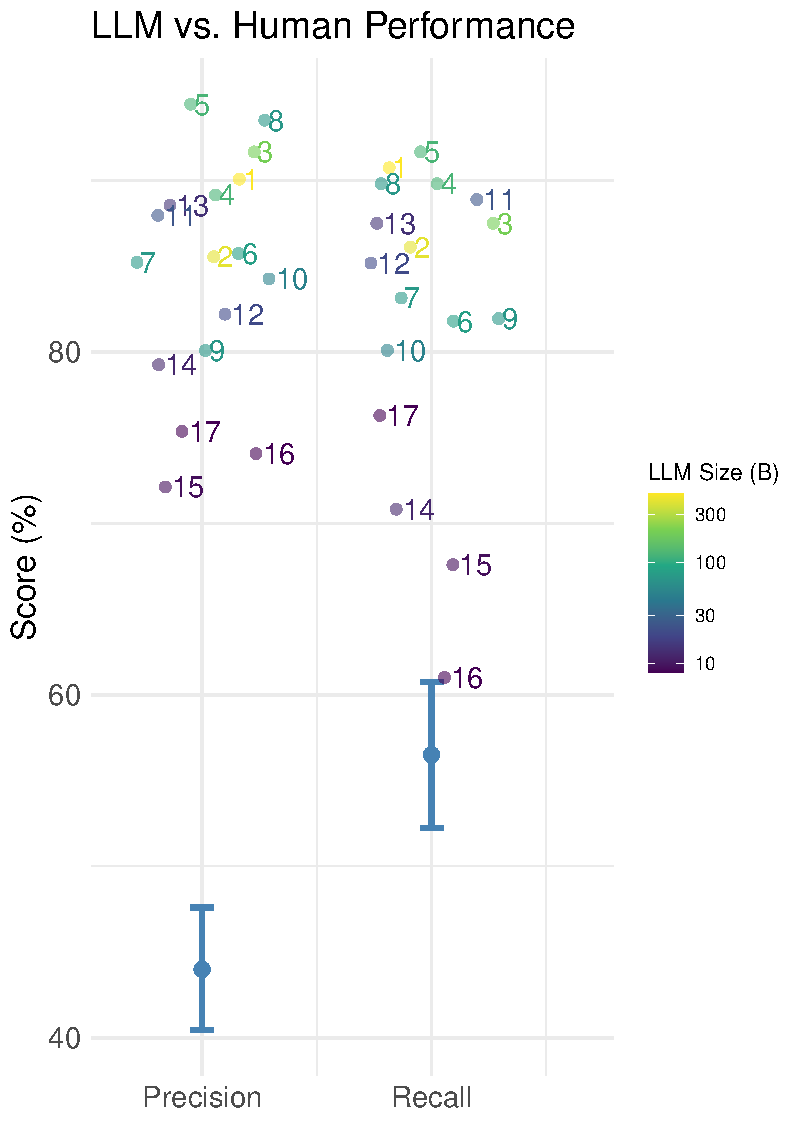
\includegraphics[width=0.8\columnwidth]{img/iRL-fig-ci.plot.pdf} 
\caption{95\% confidence interval of mean human performance and performance data of individual LLMs (dots).}\label{fig:ci}
\end{figure}


In accordance with our research questions, the null hypotheses (whose rejection is attempted) are as follows:

\textbf{H$_0^1$.} For each LLM, performance falls within the 95\% confidence interval of the average human performance, measured in terms of per-participant precision and recall --- $\mathrm{prec}^{pp}_V(p)$ and $\mathrm{rec}^{pp}_V(p)$.

\textbf{H$_0^2$.} Model size does not have a relationship with performance in terms of, again accuracy. 

To attempt to reject H$_0^1$, we form the corresponding confidence interval and check if the precision and recall of each LLM falls within the interval. To reject H$_0^2$ we perform a simple regression using model size as predictor and the F1 score (harmonic mean of precision and recall) as response variable. 

\subsection{Results}

\begin{table}
\centering
\caption{\label{tab:dems}Participant Counts and Ages by Sex and Case.}
\centering
\begin{tabular}[t]{llrr}
\toprule
Case & Sex & Average Age & Count\\
\midrule
 & Female & 33 & 8\\

\multirow{-2}{*}{\raggedright\arraybackslash Manufacturing} & Male & 34 & 12\\
\cmidrule{1-4}
 & Female & 32 & 5\\

\multirow{-2}{*}{\raggedright\arraybackslash Thermostat} & Male & 30 & 10\\
\bottomrule
\end{tabular}
\end{table}

\subsubsection{Participation}

Of the forty (40) participants invited, five (5) disqualified due to a low score in the video comprehensibility questions. This resulted in a total of thirty-five (35) usable cases. The statistics in terms of case they worked on, sex, and age can be found in Table \ref{tab:dems}. Of the 19 LLMs, all but two small ones (\textit{meta-llama/llama-3.2-1b-instruct} and \textit{google/gemma-3-4b-it}) gave usable output resulting in 17 performance data points in total.



\subsubsection{Outcome}

The LLMs achieved higher performance than humans overall. Table \ref{tab:medians} shows the median precision and recall values for Humans and LLMs, accounted per concept and per participant. Furthermore, we consider the 35 data human points and create studentized bootstrap confidence intervals for precision and recall (bootstrap-t method; R = 999 iterations) at the 95\% confidence level. The intervals can be viewed in Figure \ref{fig:ci} along with labeled dots representing the corresponding performance of each LLM. All LLM points fall outside the 95\% confidence interval, meaning that for each LLM, we reject the null hypothesis \textbf{H$_0^1$} that its precision and recall are equal to the human population mean ($\alpha$ = 0.05). Thus, by the standard that we set above for justifying  substitutability of humans by LLMs, none of the LLMs can play that specific role: they are too well-performing to be representative of human performance. An alternative visualization can be viewed in Figure \ref{fig:scatter}, where the performance of individual human and LLM participants are plotted.

\begin{table}[ht]
  \centering
  \caption{Median Precision and Recall for Humans and LLMs.}
  \label{tab:medians}
  \begin{tabular}{llrr}
    \toprule
    & & Human & LLM \\
    \midrule
    \multirow{2}{*}{Per-concept}     & Precision & \input{src/iRL-pc-human-prec} & \input{src/iRL-pc-llm-prec} \\
                                     & Recall    & \input{src/iRL-pc-human-recl} & \input{src/iRL-pc-llm-recl} \\
    \midrule
    \multirow{2}{*}{Per-participant} & Precision & \input{src/iRL-pp-human-prec} & \input{src/iRL-pp-llm-prec} \\
                                     & Recall    & \input{src/iRL-pp-human-recl} & \input{src/iRL-pp-llm-recl} \\
    \bottomrule
  \end{tabular}
\end{table}

To answer whether model size affects performance, a simple linear regression was conducted with log-transformed model size as the predictor and F1 score as the response variable. A significant positive effect of model size was found ($\beta$ = 0.09, SE = 0.02, t(15) = 3.93, p = 0.001, standardized $\beta$* = 0.71){} indicating that larger models tend to perform substantially (as per effect size $\beta^*$) better in terms of F1, rejecting thereby \textbf{H$_0^2$}. Adding to this evidence, recall that the two models that failed were of size 1 and 4 Bn parameters, i.e., comparatively small. Figure \ref{fig:linear} visualizes the effect.

\begin{figure}[th]
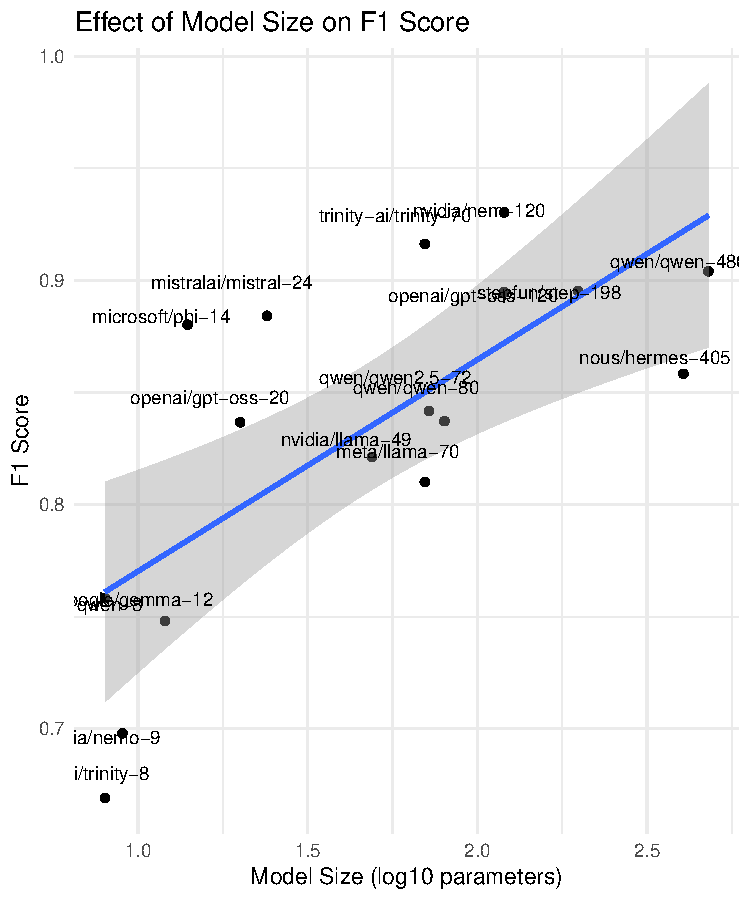
\includegraphics[width=0.95\columnwidth]{img/iRL-llm-fig-linear.pdf} 
\caption{F1 score vs. model size. The shaded band represents the 95\% confidence interval of the regression line.}\label{fig:linear}
\end{figure}

\begin{figure}[th]
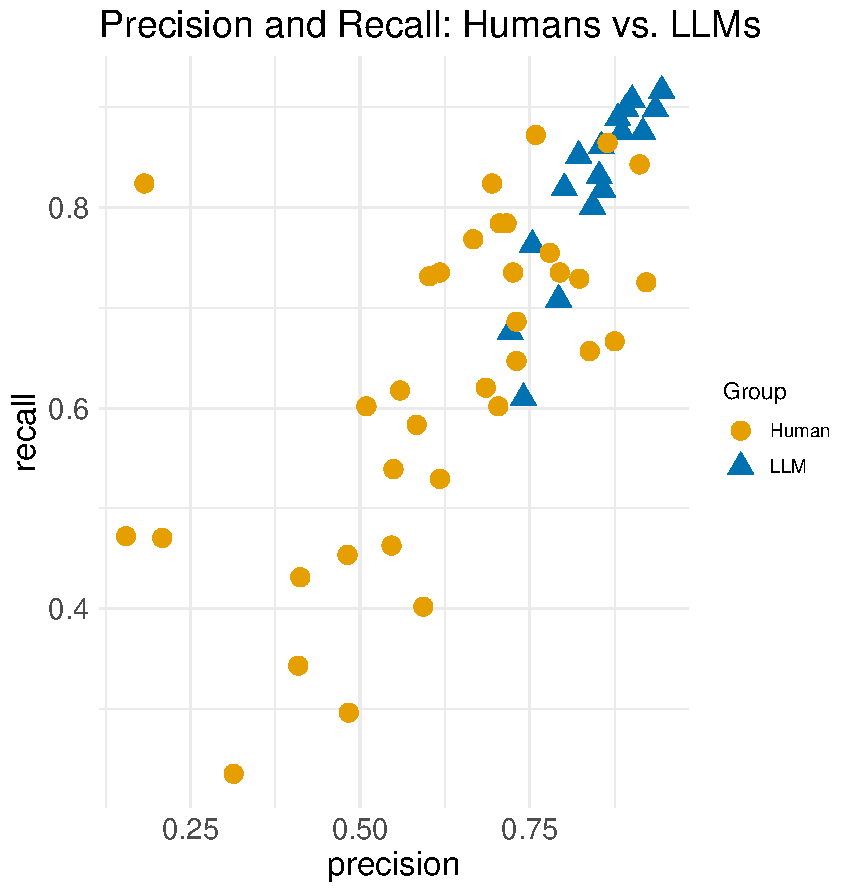
\includegraphics[width=0.85\columnwidth]{img/iRL-fig-scatter.pdf} 
\caption{Human vs. LLM performance}\label{fig:scatter}
\end{figure}





\section{Related Work}\label{sec:related}

The Peira framework we adopted in this study is part of a wider discourse in the research community on conceptualizing and evaluating model and modeling language qualities. While early frameworks for conceptually organizing the dimensions of quality, such as by Lindland et al. \cite{LiSS.94} had a strong focus on the quality of models, later proposals also explored appropriateness dimensions of the languages/grammars used to develop the models \cite{Krog.12,NePG.12,Mood.09,WaWe.93,Guiz.05}. The role of empirical studies, and particularly experiments, in assessing such qualities has also been recognized as evident by both the numerous studies published over the past decades (e.g., \cite{CGHM.13,LiHJ.13,HBKPRS.13,AlZL.17,LiRZ.17,LiTa.19} for models akin to iStar/iStar-DT alone) and the efforts to develop guidelines for systematically conducting such empirical evaluations and avoiding pitfalls \cite{BuWW.09,PaCo.05,KGPP.02,Mood.05,HoFL.12}. Peira is the outcome of a longer-term effort \cite{LiJa.20,LiMK.21b} to offer specific and readily executable data collection and analysis procedures and artifacts, based on metrics that are direct operationalizations of established theories of language quality.  

Since the advent of LLMs, research has emerged investigating their role in assisting with conceptual modeling tasks, primarily automated model generation. Studies have been conducted for a variety of languages including UML (e.g., \cite{CTBV.23,DGCT+24,FeAA.24,XiSB.25}), BPMN (e.g., \cite{HoMR.26,LPRM.25,NAAD+25,WWLL+24}) and goal models \cite{CCHY+23}. More relevant to our work is the investigation of LLMs in assisting with model quality. Gutschmidt and Nast \cite{GuNa.25}, for instance, use an LLM to evaluate aspects of model quality, referring to the SEQUAL quality framework \cite{Krog.12}, while Ayad and AlSayoud \cite{AyAl.24} explore the use of GPT-4 for eliciting business process model improvements. We could not find work comparing human and LLM performance in evaluations of language vocabularies using Peira or otherwise.


\section{Concluding Remarks and Future Plans}\label{sec:conclusions}

We reported on an experimental study exploring the suitability of LLMs as substitutes for human participants in evaluating the quality of language vocabularies according to a proposed methodology, Peira. We constructed a data collection instrument intended for humans, reproduced it in the form of an LLM prompt containing the same information, and administered each to a group of humans and a group of LLMs, respectively. We found that LLM performance level is too distant from that of humans to allow the former to be used as a substitute for the latter, and that performance tends to improve as model size increases in number of parameters. 

The result opens many research questions and opportunities for future investigation. One such question pertains to finding explanations for the result, i.e., why humans perform worse than LLMs even when both groups are given the exact same information and both arguably have the preparation to comprehend that material. One explanation points to the quality of the voice and visuals in the training video or the layout of the instrument, which participants may find confusing or unstimulating. An additional, perhaps more credible, concern is that the online participants, despite having self-reported information technology education at the university or college level, may lack the specific interest or background in matters pertinent to iStar-DT. However, one can counter-argue that concepts such as \textit{goal}, \textit{effect}, \textit{wants-to} are readily comprehensible by an even wider population than the one from which our participants were sampled. Regardless, such concerns may be construed, respectively, as \textit{internal} and \textit{external validity} threats to our study and will need follow-up investigations to be resolved. 

Furthermore, the observed human vs. LLM performance gap inspires us to ask what level, if any, of training effort, intensity, detail, and care suffices for motivated humans to reach LLM-level performance. This, in turn, leads us to rethink how processes like Peira are to be utilized. Assuming that the performance of powerful LLMs offers a vocabulary comprehension standard, then Peira, when applied to humans, can be used to measure the \textit{learnability} of the vocabulary or the quality of the training process, rather than the quality of the vocabulary itself. In the iStar-DT case, for example, we could assume that its vocabulary is as well-designed as LLM ratings imply it is, and attribute the discrepancy with human data to low learnability. This would imply that the designers may either call the vocabulary successful but caution that it needs extensive training (surely more than what LLMs require), or re-engineer it to make it more learnable, which may, however, imply expressiveness-suppressing decisions, such as reducing the size of the vocabulary through concept abstraction. Nevertheless, the premise of the above reasoning, i.e., that LLMs offer a standard of comprehension of a language that any future human user can attain if they just receive enough training, needs itself to be tested and qualified. We plan to design and conduct studies that clarify if such reasoning is valid. 

We are also interested in acquiring a more complete picture of how LLMs can assist with the assessment of vocabulary quality. For example, self-reported metrics such as of semantic overlaps, and of construct deficits and excesses, which Peira elicits from humans, can be investigated when provided by LLMs vis-\`{a}-vis their relevance and validity, through, for example, expert assessment. We also plan to explore whether qualitative feedback and advice from LLMs can be useful in improving the language. 

As a final remark, in conceptualizing future work on modeling language quality assessment in general, it is relevant to acknowledge that in a world where LLM agents are also, alongside humans, producers and users of models in practical production environments, LLMs become consumers of quality as well. They are, hence, additional stakeholders to satisfy in designing the language and its training process and material. Developing systematic empirical evaluation practices tailored to LLMs is, thus, another direction for future investigation.







\begin{comment}
%%
%% The acknowledgments section is defined using the "acks" environment
%% (and NOT an unnumbered section). This ensures the proper
%% identification of the section in the article metadata, and the
%% consistent spelling of the heading.
\begin{acks}
To Robert, for the bagels and explaining CMYK and color spaces.
\end{acks}


\section*{Ethics and Privacy Statement}

This section of your ACM work should discuss the potential societal
risks that might result from its publication; two to three sentences
related to the findings of your study, or new advancements made
possible by their developed methods. The privacy and ethics statement
should clearly address the broader impacts of their work as it relates
to the authors' interpretation of privacy, fairness, safety, human
rights, data sovereignty, or future misuse and any benefit/risk
trade-off resulting from this research. We acknowledge that some
papers may have minimal societal risks beyond those considered by
institutional review boards, and the dimensions considered by any
review of the user study design or dataset licenses could be provided
in this statement.

\end{comment}

%%
%% The next two lines define the bibliography style to be used, and
%% the bibliography file.
\bibliographystyle{ACM-Reference-Format}
\bibliography{bib/biblio.bib}

\begin{comment}
%%
%% If your work has an appendix, this is the place to put it.
\appendix

\section{Research Methods}

\subsection{Part One}

Lorem ipsum dolor sit amet, consectetur adipiscing elit. Morbi
malesuada, quam in pulvinar varius, metus nunc fermentum urna, id
sollicitudin purus odio sit amet enim. Aliquam ullamcorper eu ipsum
vel mollis. Curabitur quis dictum nisl. Phasellus vel semper risus, et
lacinia dolor. Integer ultricies commodo sem nec semper.

\subsection{Part Two}

Etiam commodo feugiat nisl pulvinar pellentesque. Etiam auctor sodales
ligula, non varius nibh pulvinar semper. Suspendisse nec lectus non
ipsum convallis congue hendrerit vitae sapien. Donec at laoreet
eros. Vivamus non purus placerat, scelerisque diam eu, cursus
ante. Etiam aliquam tortor auctor efficitur mattis.

\section{Online Resources}

Nam id fermentum dui. Suspendisse sagittis tortor a nulla mollis, in
pulvinar ex pretium. Sed interdum orci quis metus euismod, et sagittis
enim maximus. Vestibulum gravida massa ut felis suscipit
congue. Quisque mattis elit a risus ultrices commodo venenatis eget
dui. Etiam sagittis eleifend elementum.

Nam interdum magna at lectus dignissim, ac dignissim lorem
rhoncus. Maecenas eu arcu ac neque placerat aliquam. Nunc pulvinar
massa et mattis lacinia.

\end{comment}

\end{document}
\endinput
%%
%% End of file `sigconf.tex'.
